\documentclass[a4paper, 1]{article}
\usepackage{lmodern}
\usepackage{amssymb,amsmath}
\usepackage{bm}
\usepackage{upgreek}
\usepackage{enumitem}
\usepackage{ifxetex,ifluatex}
\usepackage{fixltx2e}
\usepackage[margin=2.54cm]{geometry}
\usepackage{mathspec}
\usepackage{pifont}
\usepackage{dcolumn}
\usepackage{tocloft} % must go before subfig
\usepackage{subfig}
\usepackage{booktabs}
\usepackage{tabularx}
\usepackage{array}
\usepackage{ragged2e}
\usepackage{xfrac}
\usepackage{threeparttable}
\usepackage{threeparttablex}
\usepackage{multirow}
\usepackage{siunitx}
\usepackage{setspace}
\usepackage{longtable,booktabs}
\usepackage{parskip}
\usepackage[titletoc,title]{appendix}
\usepackage{titletoc}
\usepackage{color}
\usepackage{tabu}
\usepackage{multirow}
\definecolor{darkblue}{rgb}{0.0,0,.6}
\definecolor{maroon}{rgb}{0.68,0,0}
\definecolor{carageen}{rgb}{0,0.369,0.086}
\usepackage{lscape}
\usepackage{rotating}
\usepackage{etoolbox}

\usepackage{hyperref}
\hypersetup{unicode=true,
            pdftitle={The gender gap in UK academic economics 1996--2018: progress, stagnation and retreat},
            pdfauthor={},
            pdfborder={0 0 0},
            breaklinks=false,
            hypertexnames=false,
            colorlinks,
            citecolor=darkblue,
            linkcolor=maroon
            }

% Natbib
\usepackage{natbib}
\bibliographystyle{0-templates/OEconomia_EN_2}
\renewcommand{\bibsection}{}

% SI setup
\sisetup{
  input-symbols=(),
  table-align-text-post=false,
  input-decimal-markers={.},
  group-digits=integer,
  round-mode=places,
  round-precision=3,
  tight-spacing=true,
  group-separator={},
  group-minimum-digits=4,
  table-format=5.4}

% Spacing
\setstretch{1.2}
\setlength{\abovecaptionskip}{15pt plus 3pt minus 2pt}
\setlength{\belowcaptionskip}{5pt plus 3pt minus 2pt}

% Table notes fontsize.
\appto\TPTnoteSettings{\footnotesize}

% TOC format
\renewcommand*{\cftsecdotsep}{4.5}  % use dots in the section entries
\setcounter{tocdepth}{4}

% Appendix name.
\renewcommand\appendixname{Appendices}
\renewcommand\appendixpagename{Appendices}

% Landscape
\newcommand{\blandscape}{\begin{landscape}}
\newcommand{\elandscape}{\end{landscape}}

% This is required for pandoc.

% Shortcuts
\newcommand{\vect}[1]{\mathbf{#1}}


\let\BeginKnitrBlock\begin \let\EndKnitrBlock\end

\DeclareGraphicsExtensions{%
    .pdf,.PDF,%
    .png,.PNG,%
    .jpg,.jpeg}

\date{December 2022}
\def\square{{\Box}}
\title{\LARGE{The gender gap in UK academic economics 1996--2018: progress, stagnation and retreat}\thanks{All errors are our own. We are especially indebted to Almudena Sevilla for supporting the project, two anonymous referees and Danula Kankanam Gamage and Xianyue Liu for excellent research assistance. We also thank current and former members of the Royal Economic Society Women's Committee---and in particular Heather Joshi, Karen Mumford, Denise Osborn, Almudena Sevilla and Sarah Smith---for extensive comments and feedback on an earlier draft. Parts of this paper were originally released as a report to the Royal Economic Society's Women's Committee, titled ``The Gender Imbalance in UK Economics'', co-authored with Danula Kankanam Gamage and Xianyue Liu. The data copyright is held by the Royal Economic Society and the Higher Education Statistics Agency (HESA). Neither HESA Limited nor HESA Services Limited are responsible for any inferences or conclusions derived by the authors from the data or other information supplied by HESA Limited or HESA Services Limited.}}
\author{\onehalfspacing
  Victoria Bateman\thanks{University of Cambridge, \href{mailto:vb295@cam.ac.uk}{\nolinkurl{vb295@cam.ac.uk}}.} \and Erin Hengel\thanks{London School of Economics, \href{mailto:erin.hengel@gmail.com}{\nolinkurl{erin.hengel@gmail.com}}.}
}
\renewcommand\abstractname{\normalfont\textsc{Abstract}}

\begin{document}
\maketitle

\begin{abstract}
\noindent This paper reports on women's representation in UK economics over the last quarter century. While progress has been made, women in 2018 were still only 32 percent of economics undergraduate students and 26 percent of academic economists. Our data also suggest several areas of stagnation and retreat. First, the percentage of female UK nationals studying economics is low and falling over time. Second, female economists are substantially more likely to be employed at lower academic ranks and in fixed-term---and generally lower status---teaching- and research-only positions. Third, the representation of women is especially low among ethnic minorities studying for an economics Ph.D.~And finally, the percentage of economics professors with Asian ethnicity who are women has been falling over time, and at no point between 2012--2018 was a Black female professor of economics employed anywhere in the UK.

\vspace{1cm}
\noindent\textsc{Keywords}: Gender, Diversity, Labour Market Equality;\\
\textit{JEL}: A11, I23, J24, J44.
\end{abstract}

\pagenumbering{gobble}
\clearpage
\pagenumbering{arabic}

\clearpage

% \hypertarget{sec:introduction}{%
% \section{Introduction}\label{sec:introduction}}

At the 1971 meeting of the American Economic Association (AEA), it was declared that ``economics is not exclusively a man's field''. Alongside this declaration, a commitment was made to ``a positive program to eliminate sex discrimination among economists'' and the Committee on the Status of Women in the Economics Profession (CSWEP) was established \citep{Cherrier2017}. Similar organisations and committees have since emerged elsewhere, including the International Association for Feminist Economics (established in 1992), the UK's Royal Economic Society (established in 1996) and the European Economic Association Women's Committee (established in 2003).

A goal of many of these organisations has been to regularly report on the status of women in economics in their respective countries or regions. To fulfil this responsibility, the UK's Royal Economic Society (RES) surveyed UK departments throughout the period between 1996--2016. In this paper, we append this survey data to administrative data on all staff and students at UK higher education institutes supplied by the Higher Education Statistical Agency (HESA). Our combined dataset provides a comprehensive and intersectional overview of how diversity in economics---from the undergraduate through to the professorship levels---has evolved in the UK over the past quarter century.

While progress has been made, we find that women are still under-represented in UK academic economics at both ends of the pipeline---at the undergraduate level and among academics. In 2018, women represented 32 percent of economics undergraduate students (compared with 27 percent in 1996) and 26 percent of academic economists (compared with no more than 18 percent in 1996) \citep{Mumford1997, Tenreyro2017}. Women are, however, better represented among graduate students (around half in 2018 were women compared with 30 percent in 1996), largely thanks to an inflow of international students studying on taught master's courses.

Among students in general, we find that the representation of women is poor among UK nationals, and our data suggest that this gender gap has become worse rather than better since 2002. The proportion of UK-domiciled economics undergraduates who are women has fallen from 31 percent in 2002 to 27 percent in 2018; at the master's degree level, the proportion has fallen from 37 percent in 2002 to 31 percent in 2018. At both levels of study, women are better represented among economics students from ethnic minorities; however, the reverse is true at the Ph.D.~level. For undergraduates in 2018, the percentage of women is highest among Asian (31 percent) and Black students (33 percent) and lowest among white students (25 percent). Women's representation at the master's degree level was 5 percentage points higher among Black and minority ethnicity (BME) students than it was among non-BME students. For Ph.D.~students, however, women's representation was 10 percentage points higher among non-BME students than it was among BME students.

Among academic economists, we find that women are worse off on almost every dimension considered. They are substantially more likely to be employed at lower academic ranks---for example, in 2018, they made up 33 percent of lecturers, 27 percent of senior lecturers/readers (a category which consists of academics who rank somewhere between the lecturer and professor level) and a mere 15 percent of professors (the highest-ranking academic position). And while the overall growth in women's representation is upward, progress in closing the gender gap stalled around 2012, particularly among lecturers and professors. Compared to men, women are also more likely to be employed in fixed-term---and generally lower status---teaching-only and research-only positions.

When we look at the intersection of gender and race amongst academics, we find further reasons to be concerned. Only 8 percent of standard academic contracts were held by Black and minority ethnicity women in 2018---compared to 17 percent for men---and strikingly, at no point between 2012--2018 was a Black female professor of economics employed anywhere in the UK. Finally, the percentage of economics professors with Asian ethnicity who are women has in fact been falling (from 22 percent in 2012 to 16 percent in 2018).

Our paper adds to a growing body of research on the gender gap in economics. The gap is visible in a number of countries and across multiple dimensions. Initial research focussed on women's presence amongst academic economists, a tradition we continue here, albeit with a much more intersectional focus.\footnote{See also \citet{Blackaby2000} and \citet{Advani2020}.} Recent research has also explored women's presence in publications and textbooks \citep{Moon2022, Hengel2022, Sarsons2021, Stevenson2018}---which, by comparison with academic posts, suggests even greater under-representation---as well as seminars \citep{Doleac2021}. In addition to women's representation, the literature has also considered the degree to which women progress in the discipline relative to men, examining gender gaps in pay, tenure and promotion.\footnote{This includes, but is not restricted to \citet{Auriol2022}, \citet{Blackaby2005}, \citet{Ceci2014}, \citet{Chevalier2021}, \citet{CostaDias2021}, \citet{Gamage2020}, \citet{Ginther2004}, \citet{Kahn2020}, \citet{Lundberg2019}, \citet{Mumford2019} and \citet{Ward2001}.}

While this body of research identifies ``missing women'' in economics, a complementary literature in the history of economic thought points to a parallel problem of ``hidden women''. The contributions made by numerous female economists over the long span of the discipline---some of whom were side-lined or neglected by mainstream economics and therefore often found in non-economics departments---are now, as a result, being highlighted afresh \citep[see, \emph{e.g.},][]{Folbre1988, Kuiper2022, Madden1993, Madden2018}. While the present paper does not investigate female economists' presence in non-economics departments, we hope the issue can be examined more closely in future research.

In what follows, Section \ref{sec:setting} discusses the institutional context behind UK academia. In Section \ref{sec:data}, we describe our data. Section \ref{sec:findings} presents our findings. In Section \ref{sec:discussion} we compare our findings for the UK to other countries and consider some possible causes for the stagnation and retreat experienced in the UK and elsewhere. Section \ref{sec:conclusion} concludes.

\hypertarget{sec:setting}{%
\section{UK academia}\label{sec:setting}}

The UK is home to around 170 universities. The oldest English universities are Oxford and Cambridge, which were established in the 12th and 13th centuries, respectively. The first universities in Scotland were St Andrews, Glasgow, Aberdeen and Edinburgh, all founded in the 15th and 16th centuries. Most other well-known UK universities date from the 19th and early 20th centuries, with the notable exception of around 40 former polytechnic teaching institutions (many originally founded in the 1960s) that were granted university status in 1992.

UK universities are legally independent entities. Academic matters are usually overseen by a senate composed of a university's academic staff; non-academic affairs---including finances, estate management and human resources---are generally governed by a council of lay members. Most universities' revenue is a mix of tuition fees and government spending. The latter is generally tied to student numbers, subjects taught and the quality and volume of research; the former is capped for most UK students but can run as high as £60,000 per year for international students \citep[see, \emph{e.g.},][]{Cambridge2022}.

There are four academic ranks in UK universities. ``Lecturers'' are traditionally entry-level positions analogous to assistant professors in the United States; the next rank, ``senior lecturer'', is roughly equivalent to an associate professor. The third rank, ``reader'', is awarded to distinguished senior academics who have not yet attained the status of ``professor'', which is traditionally reserved only for the most senior academics and is roughly equivalent to chaired professorships in the United States.\footnote{``Reader'' is equivalent a U.S. non-chaired professor. Some UK universities have eliminated the ``reader'' title entirely, converted it to ``professor'' or combined it with ``senior lecturer'' into a single rank (sometimes titled ``associate professor'').}

Most UK academic appointments at the level of lecturer and above combine responsibilities for both teaching and research and are made on a permanent/open-ended basis. Before 1987, academic posts were ``tenured'' following a three-year probationary period, meaning that tenured staff could not be made redundant under any circumstance (although they could still be dismissed for reasons related to competence or conduct). Tenure was abolished, however, with the Education Reform Act of 1988;\footnote{The Act technically awards universities' councils the power to make academic staff redundant. Unlike other universities in the UK, most academic staff at Oxford and Cambridge are members of these governing bodies and are therefore especially unlikely to approve any redundancy plans put before them. As a result, academic staff at both universities are, \emph{de facto}, afforded far stronger employment protections compared to academics employed by other institutions. For further information and discussion, see \citet{Otsuka2019}.} as a result, academic staff in UK universities are no longer legally protected against redundancy, and at most universities, they now have the same statutory employment rights as other workers in the UK.\footnote{Some UK universities continue to apply a three-year probationary period to new academic staff; however, the abolishment of tenure meant that dismissals due to failing probation are no longer regulated by the 1971 Academic and Related Salaries settlement between the University Authorities Panel and the Association of University Teachers \citep{AUT1974}. As a result, probationary staff members in the UK are afforded similar statutory employment protections as non-probationary staff members with the same length of service.}

\hypertarget{sec:data}{%
\section{Data}\label{sec:data}}

To analyse the gender composition of UK academic economists, we combine data from two sources: data collected by the Royal Economic Society (RES) for the period 1996--2016 and data from the UK's Higher Education Statistics Agency (HESA) for the period 2012--2018.

The RES data are from a historic survey of the members on its Conferences of Heads of University Departments of Economics (CHUDE). The survey was conducted bi-annually between 1996--2016 and provide a panel dataset of departments' gender composition by rank and year. For further discussion of the history and methodology of the survey, and for why data collection ceased in 2016, see \citet{Bateman2021}.

HESA staff data are reported by universities and cover all individuals on a contract of employment with a publicly funded higher education provider in the UK during a given academic year (1 August to 31 July). The data we analyse stratify staff numbers in terms of full-time equivalents (FTE), where FTE indicates the proportion of a full-time year being undertaken within a given stratification. For the purposes of this analysis, we restrict staff data to include only academic staff members who engage in teaching and/or research activities in the field of economics. To identify economists, we select staff members employed by an economics department or business school and whose primary or secondary academic discipline is economics. To ensure they are engaged in academic teaching and/or research activities, we additionally exclude people not on academic contracts or on atypical contracts as well as staff with an unknown academic rank, classified as professional or administrative staff and routine or simple task providers. Since our primary aim is to analyse gender differences in career academic economists, we also exclude teaching and research assistants unless otherwise mentioned.

HESA data for students include information on all students enrolled in a course with a level of instruction above three according to Ofqual's Qualifications and Credit Framework (or an earlier equivalent). The data we analyse break down student counts in terms of ``instance'', where instance refers to a particular student-course combination.\footnote{Since students can take multiple courses, a single student may correspond to more than one instance in the data. Moreover, universities can report up to three subject descriptors for each course with the proportion of time the course allocates to the subject. For example, students enrolled on a BSc programme that devotes equal time to philosophy and economics would appear as two instances in the HESA data, each weighted by 0.5.} We restrict the data to men and women enrolled full-time on a standard economics degree programme. As a result, we exclude part-time and other non-full-time students and those on non-first-degree undergraduate programmes or non-master's/Ph.D.~postgraduate programmes. Given the purpose of this exercise is to analyse the representation of women in economics, our focus is on those who declare their gender as either male or female.\footnote{We hope less restrictive, binary classifications will be explored in future research.}

Published research using HESA data must comply with its rounding and suppression strategy. To adhere to this strategy, all counts of people are rounded to the nearest multiple of five and percentages are suppressed if they are based on fewer than 22.5 individuals. Because these rules are applied post-calculation (\emph{e.g.}, after summing FTEs), numbers may not always perfectly add up (\emph{e.g.}, the counts of male and female students may not precisely sum to the total number of students in a category). Further details of HESA's rounding and suppression strategy can be found on its website.

\hypertarget{sec:findings}{%
\section{Findings}\label{sec:findings}}

\hypertarget{sec:staff}{%
\subsection{Academic staff}\label{sec:staff}}

\hypertarget{sec:contract-level}{%
\subsubsection{Academic rank}\label{sec:contract-level}}



\begin{table}

\caption{\label{tab:contract}UK academic economists in 2018, by academic rank}
\centering
\begin{threeparttable}
\begin{tabular}[t]{lrrrrrr}
\toprule
\multicolumn{1}{c}{} & \multicolumn{4}{c}{ } & \multicolumn{2}{c}{Dist. across rank} \\
\cmidrule(l{3pt}r{3pt}){6-7}
Academic rank & Male & Female & Total & \% female & Male (\%) & Female (\%)\\
\midrule
Lecturer (A) & 85 & 60 & 145 & 40 & 7 & 13\\
Lecturer (B) & 420 & 185 & 610 & 31 & 33 & 41\\
Reader/SL & 365 & 135 & 505 & 27 & 29 & 30\\
Professor & 400 & 75 & 475 & 15 & 31 & 16\\
\midrule
Total & 1,275 & 455 & 1,725 & 26 & 100 & 100\\
\bottomrule
\end{tabular}
\begin{tablenotes}[para]
\item \textit{Note.}
\item Table displays information on economists employed on a standard academic contract (\emph{i.e.}, full-time, permanent with both teaching and research responsibilities) by a UK institute of higher education during the 2018--19 academic year. First three columns show raw FTE counts; the fourth column displays the representation of women in each rank as a percentage of the total; the fifth (sixth) column shows the distribution of men (women) by rank as a percentage of all men (women). Data from HESA.
\end{tablenotes}
\end{threeparttable}
\end{table}



In UK academic economics, women are substantially more likely to be employed at lower academic ranks. The first three columns in Table \ref{tab:contract} report the numbers of economists employed in 2018 on a ``standard'' academic contract---\emph{i.e.}, full-time, permanent contract with both teaching and research responsibilities---at a UK institute of higher education. In aggregate, 1,725 economists satisfy these employment conditions, 455 of whom are women (26 percent). Women make up 33 percent of lecturers (A and B combined), 27 percent of senior lecturers/readers and 15 percent of professors.\footnote{\label{fn:lecAB}Lecturer A positions correspond to a lower pay grade compared to lecturer B positions (see the \href{https://www.ucu.org.uk/framework}{higher education pay framework agreement}). Unless otherwise mentioned, ``lecturer'' combines both categories.}

Table \ref{tab:contract}'s final two columns display each gender's distribution across academic rank. Among all female economists employed on a standard academic contract, more than one in two are lecturers (13 percent Lecturer A and 41 percent Lecturer B), a little under one in three is a senior lecturer/reader (30 percent) and a little over one in seven is a professor (16 percent). The picture is remarkably different for men: out of every three men, roughly one is a professor (31 percent), one is a senior lecturer/reader (29 percent) and one is a lecturer (B) (33 percent). Only a small percentage of male academic economists are on lecturer A contracts (7 percent).



\begin{figure}
\centering
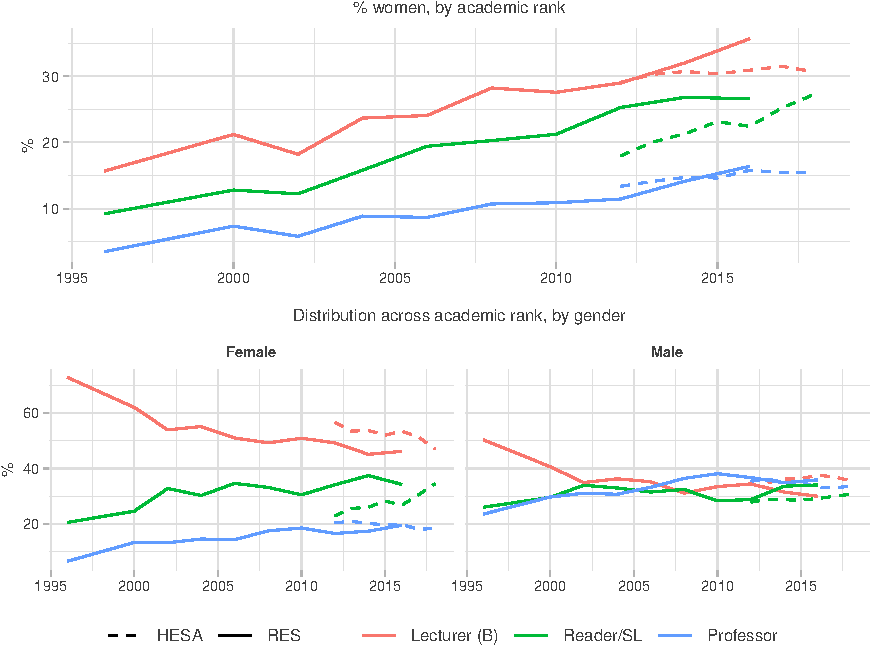
\includegraphics[width=\linewidth]{0-images/contract-1.pdf}

\caption{UK academic economists over time, by academic rank}
\label{fig:contract}
\justify\footnotesize\textit{Note}.  Top figure plots the percentage of women employed as lecturers (B lecturers, only), senior lecturers/readers and professors. Bottom graphs plot the fraction of all female economists (left) and all male economists (right) employed in each academic rank. Solid lines represent RES survey data; dashed lines are based on HESA data. Data restricted to standard academic contracts, defined as being full-time, permanent contracts with responsibilities for both teaching and research. Data from HESA and RES.
\end{figure}



The overall growth in women's representation in economics is upward, but seems to have stalled since 2012, particularly among lecturers and professors. Figure \ref{fig:contract}'s top graph plots the percentage of women employed in lecturer B positions (red), as senior lecturers/readers (green) and as professors (blue); solid and dashed lines represent RES survey data and HESA data, respectively.\footnote{\label{fn:lecA}To ensure RES survey and HESA samples are as similar as possible, we omit lecturer A positions from the HESA data and include only lecturers with permanent positions from the RES survey data.} In 1996, approximately 3 percent of professors, 9 percent of senior lecturers/readers and 16 percent of lecturers were female. By 2018, these shares had increased to 15, 27 and 31 percent, respectively. For lecturers and professors, however, much of this growth occurred before 2012; after that, the percentage of women in each role increased only 1.6 and 2.0 percentage points, respectively. Women's representation among senior lecturers/readers grew much more (9 percentage points).

Temporal changes in the fraction of all men and all women at each academic rank are shown in the bottom two graphs of Figure \ref{fig:contract}.\footnote{Each graph in the second row of Figure \ref{fig:contract} displays the percentage of academic economists employed by rank in a particular year for the given gender; thus, conditional on year and gender, the percentages for each rank sum to 100.} In 1996, roughly one in every two male academics was a lecturer, one in four was a senior lecturer/reader and another one in four was a professor. As already discussed, these proportions had changed dramatically by 2018: men were about equally represented in all three categories. The 1996 position for women was vastly different---almost three quarters of female staff members were lecturers and only 1 in sixteen was a professor. And while these gaps have closed substantially, female economists in UK academia are still far more likely to be lecturers than they are to be senior lecturers/readers and, especially, professors.

Figure \ref{fig:contract} allows us to compare HESA data with the RES survey data collected between 1996--2016. In all three graphs, HESA data for professors tracks the RES survey data closely during the overlapping period (2012--2016). But compared to the HESA data, the RES survey data over-estimates the fraction of senior lecturers/readers who are women and under-estimates the fraction of lecturers who are women. These differences, however, are relatively minor; both data sources suggest similar conclusions about the representation of female economists in UK academia.\footnote{These discrepancies are caused by small variations in the institutions covered by each dataset as well as differences in how posts are categorised.}

\hypertarget{academic-employment-function}{%
\subsubsection{Academic employment function}\label{academic-employment-function}}



\begin{figure}
\centering
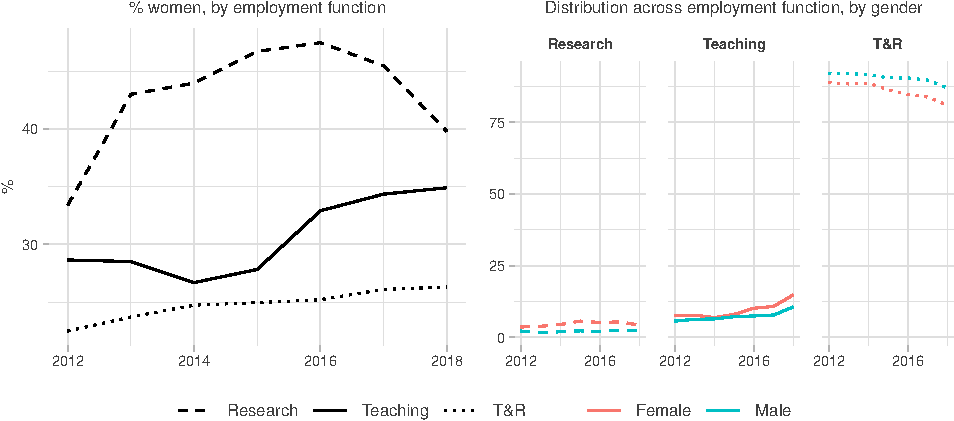
\includegraphics[width=\linewidth]{0-images/emp-function-1.pdf}

\caption{UK academic economists, by academic employment function}
\label{fig:emp-function}
\justify\footnotesize\textit{Note}.  Left-hand graph plots the percentage of women employed in teaching-only, research-only and teaching and research (T\&R) positions. Right-hand graph plots the percentages of all female economists and all male economists across employment function. Data restricted to full-time, permanent contracts held by lecturers, senior lecturers/readers and professors. Data from HESA.
\end{figure}



When we break down data by academic employment function, we find that women have been gaining ground in teaching-only and research-only positions, but have made slower progress obtaining more traditional (and generally more prestigious) positions with both responsibilities (Figure \ref{fig:emp-function}, left-hand graph).\footnote{Teaching-only positions make-up 3 percent of people working in economics academia on a full-time permanent contract; research-only positions make up a further 12 percent. The remaining 85 percent have responsibilities for both teaching and research.} Between 2012--2018, the representation of women among academic economists employed on a permanent, full-time basis at lecturer-level or above but with only teaching or research responsibilities increased 6.3 and 6.4 percentage points, respectively; the corresponding figure for teaching and research (T\&R) positions was just 4 percentage points.

Women are (in relative terms) over-represented in teaching- and research-only positions and under-represented in most positions that combine both responsibilities (Figure \ref{fig:emp-function}, right-hand graph). The share of women among T\&R staff is consistently lower than the corresponding share for men---in 2018, 81 percent and 87 percent, respectively, for a difference of 6 percentage points. Worryingly, this gap has \emph{widened} over time. (In 2012, it was only 3 percentage points.) Meanwhile, the proportion of all women in teaching only positions (15 percent) is greater than the proportion of all men in those same positions (11 percent), meaning a greater fraction of female academic economists are employed on teaching-only contracts compared to men. Again, this gap has been increasing (in magnitude) over time: in 2012, teaching-only appointments were 2 percentage points more common among women; by 2018, that difference had increased to 4 percentage points. Women are also slightly over-represented among research-only positions, but the gap between genders has remained relatively constant over time.

As expected, women make up a greater fraction of all three employment functions at lower academic ranks. Since the percentage of women in T\&R positions is described in Section \ref{sec:contract-level}, we focus on teaching-only and research-only positions here. In 2018, women constituted 39 percent of teaching-only lecturer positions and 24 percent of teaching-only senior lecturers/readers and professors. Among research-only contracts, women made up 38 percent of lecturer positions. The numbers of senior lecturers, readers and professors on research contracts is negligible.

\hypertarget{part-time-employment}{%
\subsubsection{Part-time employment}\label{part-time-employment}}



\begin{figure}
\centering
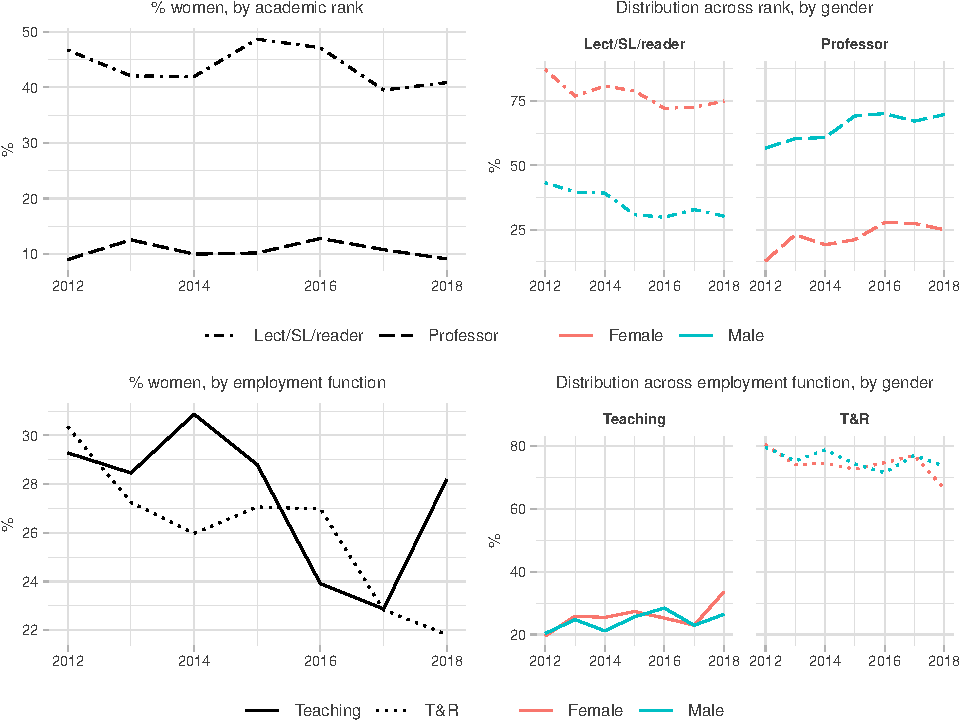
\includegraphics[width=\linewidth]{0-images/part-time-1.pdf}

\caption{UK academic economists working part-time, by academic rank and employment function}
\label{fig:part-time}
\justify\footnotesize\textit{Note}.  Top left-hand graph plots the percentage of part-time academics who are women, broken down by academic rank; the top right-hand graph plots the fraction of all part-time female and male economists across academic rank. Bottom left-hand graph plots the percentage of part-time academics who are women, broken down by academic employment function; the bottom right-hand graph plots the fraction of all part-time female and male economists across academic employment function. Data restricted to lecturers, senior lecturers/readers and professors on permanent contracts; top two graphs additionally restricted to T\&R positions. Data from HESA.
\end{figure}



Among economists employed on a permanent academic contract with responsibilities for both teaching and research, men in 2018 were slightly more likely than women to be working part-time (5 vs.~4 percent, respectively). In 2012, the reverse was true: 4 percent of men were working part-time whereas 6 percent of women were.

Perhaps even more surprising is how few female economists work part-time in UK academia. As the very first Women's Committee report noted ``Part-time employment has become increasingly prevalent throughout the UK labour market and is typically considered to be more popular amongst female employees. {[}\ldots{]} UK academia does not appear to follow this pattern, rather 15.7\% of academic economists work part-time and only 26.6\% of these jobs are held by women.'' \citep[pp.~8--9]{Mumford1997}.\footnote{The authors counted only 11 permanent part-time female academic economists on standard academic contracts in the UK in 1996.} Our data suggest that part-time employment among women in academic economics is still relatively rare: between 2012--2018, only about 20 women each year were employed on a part-time, standard academic contract.

The percentage of women in part-time employment is declining in academic rank (top left-hand graph in Figure \ref{fig:part-time}). In 2018, 41 percent of lecturers, senior lecturers and readers employed on a part-time basis were women; only 9 percent of part-time professors were. These figures have remained roughly stable over time.

The top right-hand graph in Figure \ref{fig:part-time} shows the distribution across rank of female and male part-time economists. Relative to women, men are consistently over-represented among part-time professors and under-represented among part-time lecturers, senior lecturers and readers.\footnote{Some departments have employed senior academics from non-UK institutions on fractional contracts in order to enhance their scores in the UK's national research evaluation exercises \citep[see, \emph{e.g.},][]{Stern2016}. This may explain the higher representation of male professors working ``part-time'' in UK economics departments.} In 2018, men on a part-time contract were least likely to be lecturers, senior lecturers or readers (30 percent); the vast majority were professors (70 percent). Part-time women, on the other hand, were most likely to be lecturers, senior lecturers or readers (75 percent); only 25 percent were professors. These patterns have not significantly changed since 2012.

Figure \ref{fig:part-time}'s bottom left-hand graph shows the percentage of part-time economists that are female by academic employment function. This figure hovers between 20 and 30 percent for both teaching-only and T\&R positions.\footnote{The numbers of men and women in part-time research-only positions is negligible and has therefore been omitted.} The right-hand graph plots the distribution across employment function; it suggests men and women working part-time are similarly distributed across teaching-only and T\&R positions. Again, these patterns have not changed substantially since 2012.

\hypertarget{sec:staff-temp}{%
\subsubsection{Temporary employment}\label{sec:staff-temp}}



\begin{figure}
\centering
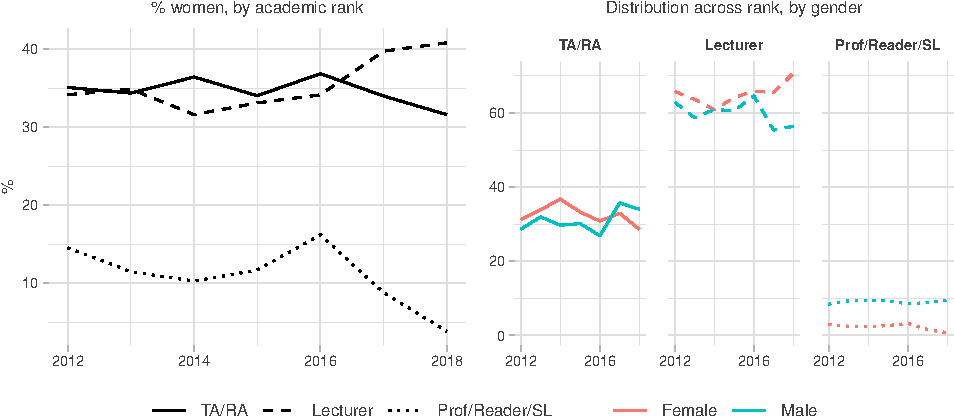
\includegraphics[width=\linewidth]{0-images/fixed-term-1.pdf}

\caption{UK academic economists on a fixed-term contract, by academic rank}
\label{fig:fixed-term}
\justify\footnotesize\textit{Note}.  Left-hand graph plots the percentage of academics on a fixed-term contract who are women, broken down by academic rank; right-hand graph plots the percentage of all women and all men on fixed-term contracts across rank. Data restricted to academic economists (including teaching/research assistants) working full- or part-time in any employment function. Data from HESA.
\end{figure}



Since 2012, there has been a slight decrease in the number and percentage of academic economists (including teaching and research assistants) employed full-time on a fixed-term contract with responsibilities for both teaching and research: in 2012, 75 economists held these jobs, or 5 percent of full-time T\&R staff; by 2018, both figures had fallen to 55 and 3 percent, respectively. The number of staff members on temporary contracts rises when teaching-only, research-only and part-time staff are included---from 420 in 2012 to 485 in 2018. As a percentage of all academic contracts, however, the use of fixed-term contracts has fallen slightly---from 19 percent of all economics staff in 2012 to 18 percent in 2018.

It appears temporary contracts are used in different ways depending on academic rank. Over the 2012--2018 period, the majority (52 percent) of professors on temporary contracts were employed in part-time T\&R positions. In contrast, fixed-term lecturers and teaching and research assistants were predominantly employed in full-time research-only positions (35 percent) and part-time teaching-only positions (31 percent). Hardly any senior lecturers and readers are employed on a fixed-term basis (2 percent in 2018).

The fraction of female economists employed in fixed-term posts exceeds their share among permanent positions. In 2018, women constituted 33 percent of staff (including teaching and research assistants) on fixed-term, full-time T\&R contracts; their corresponding share among permanent academic staff was only 26 percent.

According to the left-hand graph in Figure \ref{fig:fixed-term}, the percentage of temporary contracts held by women is highest for teaching/research assistants and lecturers (in 2018, 32 and 41 percent, respectively) and lowest for senior lecturers/readers/professors (4 percent). Figure \ref{fig:fixed-term}'s right-hand graph plots the distribution of women on fixed-term contracts across academic rank. Compared to men, women on temporary contracts are over-represented among lecturers and under-represented among senior lecturers/readers/professors. In 2012, women on a fixed term contract were slightly more likely than men to work as teaching and research assistants; by 2018, the reverse was true.

In general, the fraction of people on temporary contracts who are women is highest for teaching- and research-only positions and lowest for positions with both responsibilities (see Figure \ref{fig:fixed-term-2} in Appendix \ref{sec:temp-appendix}). Men's and women's distributions across employment function is roughly similar although men on temporary contracts are slightly more likely to be in T\&R and teaching-only positions whereas women are somewhat more likely to be in research-only positions: in 2018, 48 percent of women and 42 percent of men employed on a temporary basis held research-only positions, 41 and 43 percent were employed in teaching-only positions and 11 and 16 percent held positions with both responsibilities.

Conditional on holding a fixed-term contract, women disproportionately work full-time. In 2018, women held 38 percent of full-time fixed-term contracts but only 31 percent of part-time fixed-term contracts. Among academic staff on a fixed-term contract, 72 percent of women work full-time compared to 65 percent of men (Figure \ref{fig:fixed-term-2}, Appendix \ref{sec:temp-appendix}).

\hypertarget{nationality}{%
\subsubsection{Nationality}\label{nationality}}



\begin{figure}
\centering
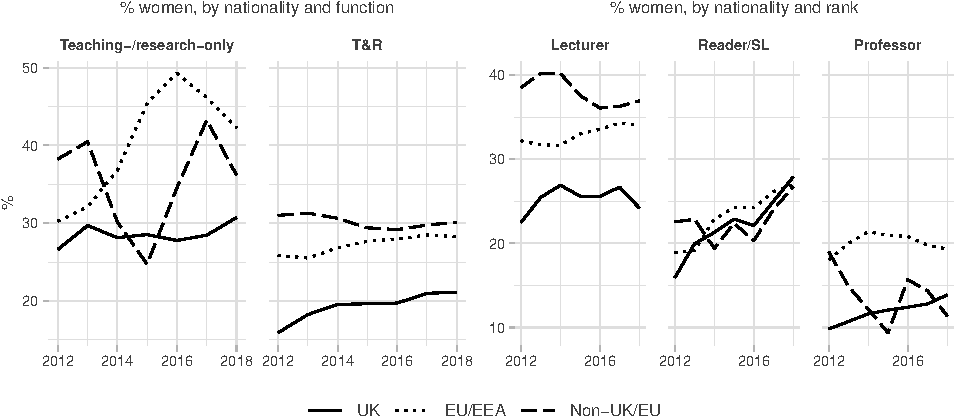
\includegraphics[width=\linewidth]{0-images/nationality-1.pdf}

\caption{UK academic economists, by nationality}
\label{fig:nationality}
\justify\footnotesize\textit{Note}.  Left-hand graph plots the percentage of women by nationality and academic employment function; right-hand graph plots the percentage of women by nationality and academic rank. Data restricted to lecturers, senior lecturers/readers and professors on permanent, full-time contracts; right-hand graph includes only academics with responsibilities for both teaching and research. Data from HESA.
\end{figure}



Almost three-quarters of female economists employed in the UK higher education system are originally from a country outside the UK. Of the 455 female economists employed in 2018 as a lecturer, senior lecturer/reader or professor on a full-time, permanent T\&R contract, only 125 were from the UK (28 percent). For comparison, of the 1,275 male economists employed in 2018 on a standard academic contract, 475 were UK nationals (37 percent).

The left-hand graph in Figure \ref{fig:nationality} plots the percentage of women by nationality and academic employment function. Women from all nationalities are better represented in research- and teaching-only positions compared to T\&R positions. In general, the representation of women is lowest among UK academics regardless of employment function. Conditional on holding a T\&R post, there are more women among non-UK/EU academic staff members (30 percent); close behind them are EU/EEA staff members (28 percent). Women only make up 21 percent of UK academic economists in T\&R positions.

Figure \ref{fig:nationality}'s right-hand graph plots the percentage of women in UK academia by nationality and rank. For lecturers, women's representation is highest among non-UK staff members (in 2018, 37 and 34 percent for non-UK/EU and EU/EEA staff members, respectively) and lowest among staff members from the UK (24 percent). For non-UK academic staff, the percentage of women falls quite a bit at the level of senior lecturer/reader (26.7 and 26.9 percent for non-UK/EU and EU/EEA staff members, respectively); for UK staff, however, women's representation among senior lecturers/readers (28 percent) is slightly higher than their representation among lecturers (24 percent). At the professorial level, the share of women drops regardless of nationality (14, 19 and 11 percent for UK, EU/EEA and Non-UK/EU staff members, respectively).

\hypertarget{ethnicity}{%
\subsubsection{Ethnicity}\label{ethnicity}}



\begin{figure}
\centering
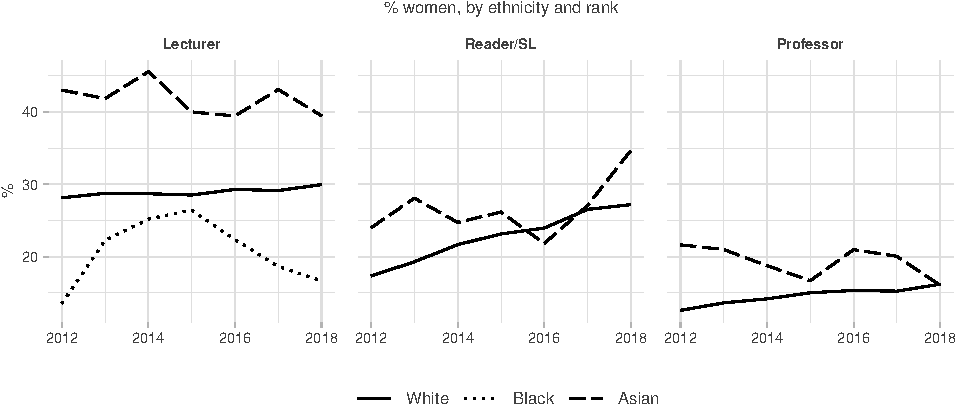
\includegraphics[width=\linewidth]{0-images/ethnicity-1.pdf}

\caption{UK academic economists, by ethnicity}
\label{fig:ethnicity}
\justify\footnotesize\textit{Note}.  Figures plot the percentage of women employed as academic economists in the UK by academic rank and ethnicity. Data restricted to permanent, full-time, T\&R contracts at the level of lecturer or above. Due to HESA's rounding and suppression strategy, we are unable to plot the percentage of women among Black senior lecturers/readers, and the number of female Black professors of economics is zero; for similar reasons (as well as to enhance readability), we also omit individuals whose ethnicity is classified as other or mixed. See Appendix \ref{sec:data-definitions} for further information on how ethnicity is categorised. Data from HESA.
\end{figure}



In 2018, 8 percent of standard academic posts in economics were held by Black and minority ethnic (BME) women. This figure is only 2 percentage points higher than it was in 2012. For comparison, BME men constituted 17 percent of all standard academic contracts in 2018, a 3 percentage point increase from 2012.

Figure \ref{fig:ethnicity} displays the percentage of female economists employed on a standard academic contract by ethnicity and academic rank.\footnote{See Appendix \ref{sec:data-definitions} for further information on how ethnicity was categorised; due to relatively small numbers and to enhance readability, individuals whose ethnicity is classified as other or mixed are not included.} Women's representation is highest among Asian individuals: in 2018, there were 155 Asian lecturers, 39 percent of whom were women. Among the 490 white lecturers, 30 percent were women. Of the roughly 25 Black lecturers in economics, however, no more than 5 (17 percent) were women.\footnote{These results are consistent with \citet{Blanco2010}, who found that in 2010, women made up 41 percent of academic economists in the UK with a Chinese background and 30 percent with a South East Asian background. Moreover, of the 121 permanently employed female economics lecturers in their data, only one was Black.}

Among those of Asian ethnicity, the percentage of women declines as academic rank increases: in 2018, there were 85 Asian senior lecturers/readers and 50 professors, 35 and 16 percent of whom were women, respectively. Among individuals with white ethnicity, however, the decline is only apparent at the professorial level: the percentage of female senior lecturers/readers is similar to that of lecturers (27 and 30 percent in 2018, respectively); the share of female professors is much lower (16 percent). Worryingly, the percentage of Asian professors who are women declined 6 percentage points---from 22 percent to 16 percent---between 2012--2018. The decline was especially stark among economists from an Indian, Pakistani and Bangladeshi background.

In 2018, there were no more than 10 Black senior lecturers/readers in economics employed on a standard academic contract, very few of whom were women. At no point between 2012--2018 was a Black female professor of economics employed anywhere in the UK according to the HESA data.\footnote{This was similarly found to be the case in \citet{Blanco2010}. We also note that our own data include only those individuals who are based in economics departments or business schools and whose primary and/or secondary research interest is economics/econometrics as defined by HESA's own subject coding. Our results may therefore omit female economists employed outside these departments or with economics-adjacent research interests (\emph{e.g.}, business management or social policy).}

Most BME academic economists employed full-time in a permanent post have responsibilities for both teaching and research (130 individuals in 2018). A much smaller number (25) were in teaching-only positions. Hardly any BME academic economists hold research-only positions.

\hypertarget{sec:students}{%
\subsection{Students}\label{sec:students}}

\hypertarget{level-of-study}{%
\subsubsection{Level of study}\label{level-of-study}}



\begin{table}[!h]

\caption{\label{tab:level}UK economics students in 2018, by level of study}
\centering
\begin{threeparttable}
\begin{tabular}[t]{lrrrrrr}
\toprule
\multicolumn{1}{c}{} & \multicolumn{4}{c}{ } & \multicolumn{2}{c}{Dist. across level} \\
\cmidrule(l{3pt}r{3pt}){6-7}
Level of study & Male & Female & Total & \% female & Male (\%) & Female (\%)\\
\midrule
First degree & 25,315 & 12,000 & 37,310 & 32 & 87 & 77\\
Master's & 3,000 & 3,220 & 6,220 & 52 & 10 & 21\\
Doctorate & 655 & 410 & 1,070 & 39 & 2 & 3\\
\midrule
Total & 28,970 & 15,630 & 44,600 & 35 & 100 & 100\\
\bottomrule
\end{tabular}
\begin{tablenotes}[para]
\item \textit{Note.}
\item Table displays information on full-time male and female students studying economics on a standard degree programme during the 2018--19 academic year at a UK institute of higher education. First three columns show raw numbers; the fourth column displays the representation of women in each level as a percentage of the total; the fifth (sixth) column shows the distribution of men (women) across level. Data from HESA.
\end{tablenotes}
\end{threeparttable}
\end{table}



In economics, women are more common among taught post-graduate students than they are among undergraduate or Ph.D.~students. Table \ref{tab:level} breaks down the number of full-time students studying economics in a British institute of higher education during the 2018--19 academic year. Total student numbers were 44,600; of them, 15,630 were women (35 percent). Women make up 32 percent of undergraduate, 52 percent of master's and 39 percent of Ph.D.~students in economics. Table \ref{tab:level}'s final two columns reinforce this conclusion. They display each gender's distribution across level of study. Compared to women, men disproportionately study economics at the undergraduate level; women disproportionately study it at the master's level. Similar proportions of male and female economics students are working toward a Ph.D.

Overall growth in women's representation among economics students is flat. Nor has there been any recent change to men's and women's distribution across level of study. At no level has there been a substantial increase (or decrease) in the percentage of women studying economics between 2012--2018 (Figure \ref{fig:level}, left-hand graph). The right-hand graph in Figure \ref{fig:level} displays the fraction of all men and all women by level of study. Men are consistently over-represented among undergraduate students of economics; women are consistently over-represented among master's students.



\begin{figure}
\centering
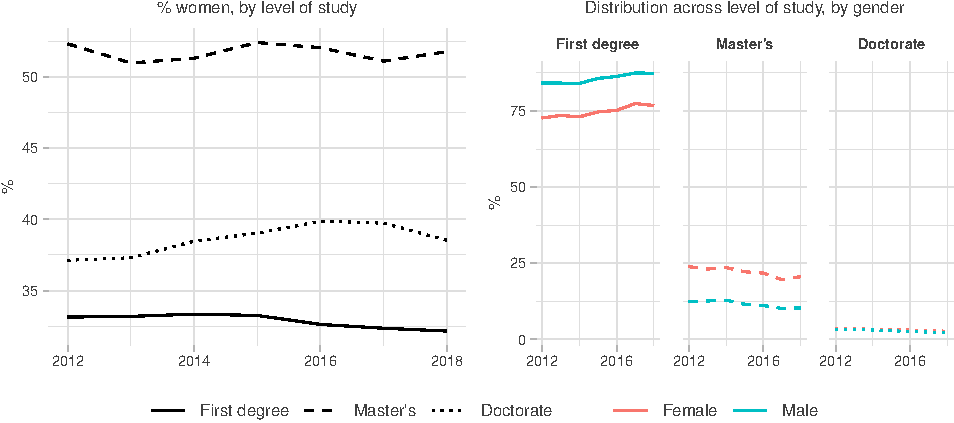
\includegraphics[width=\linewidth]{0-images/level-1.pdf}

\caption{UK economics students, by level of study}
\label{fig:level}
\justify\footnotesize\textit{Note}.  Left-hand graph plots the percentage of female students in economics by level of study; the right-hand graph displays the fraction of all female and all male economics students across level of study. Data are for full-time male and female students studying on a standard degree programme. Data from HESA.
\end{figure}



\hypertarget{domicilenationality}{%
\subsubsection{Domicile/nationality}\label{domicilenationality}}



\begin{figure}
\centering
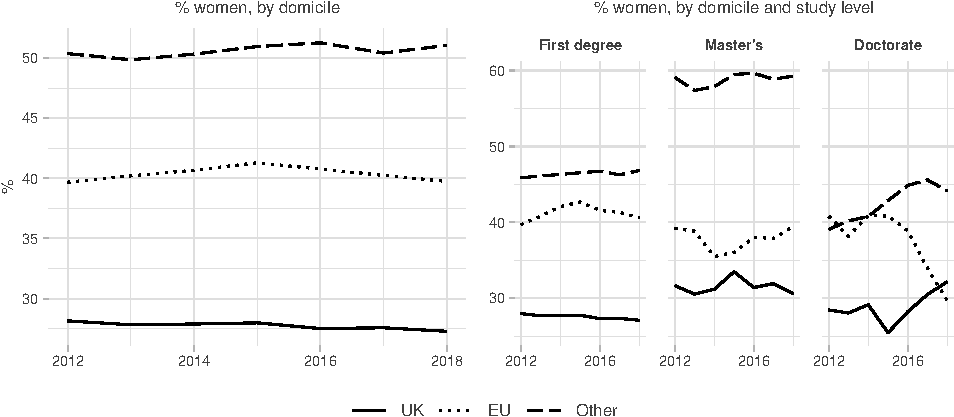
\includegraphics[width=\linewidth]{0-images/domicile-1.pdf}

\caption{UK economics students, by domicile}
\label{fig:domicile}
\justify\footnotesize\textit{Note}.  Left-hand graph plots the percentage of female students in economics by domicile; right-hand graphs plot the percentages of women, by domicile and study level. Data are for full-time male and female students studying for a standard degree programme and omit students with an unknown domicile. Data from HESA.
\end{figure}



The representation of women is especially poor among UK residents. Figure \ref{fig:domicile}`s left-hand graph plots the percentage of women studying economics full-time at a UK institute of higher education by domicile.\footnote{Domicile refers to the location of a student's permanent home address prior to starting study.} Between 2012--2018, women have consistently made up at least half of all non-UK/EU students and about 40 percent of all EU students. For the UK, however, women represented only 27 percent of economics students in 2018; if anything, this figure has slightly declined since 2012, when it was 28 percent. Conclusions are similar when considering students' nationality instead of domicile (see Figure \ref{fig:domicile-2}, Appendix \ref{sec:student-nationality}).

British women are absent from economics at every level of study. Figure \ref{fig:domicile}'s right-hand graph plots the percentage of women by study level and domicile. Among economics students domiciled in the UK in 2018, women represented 27 percent of undergraduates, 31 percent of master's students and 32 percent of Ph.D.~students. In contrast, in 2002 women were 31 and 37 percent of UK-domiciled economics undergraduates and master's students, respectively \citep{Blanco2013, Mitka2015}, suggesting that both gender gaps have been getting worse over time. There has, however, been a small improvement at the doctoral level: 28 percent of UK-domiciled economics students were women in 2002; that figure rose to 33 percent by 2011 \citep{Blanco2013} and has remained steady since.

Women's representation is higher among EU-domiciled students, but similarly stable across undergraduates and master's students---in 2018, 41 percent of EU undergraduates and 39 percent of EU master's students were women---before falling among Ph.D.~students (30 percent). Between 2012--2018, the share of women among EU Ph.D.~students declined 11 percentage points. Again, conclusions are similar when the analysis is based on nationality instead of domicile (see Figure \ref{fig:domicile-2}, Appendix \ref{sec:student-nationality}).

Across every degree level, women's representation is highest among non-UK/EU students. Indeed, women made up 59 percent of non-EU/UK students studying economics at the master's level. Thus, the over-representation of women at this level---apparent in Figure \ref{fig:level}---is clearly due to large inflows of non-UK/EU women coming to the UK to study economics on a taught postgraduate programme.\footnote{Note that non-EU/UK women make up 81 percent of all female students studying economics at the master's level.}

The top two graphs in Figure \ref{fig:secondary} (Appendix \ref{sec:secondary}) break down the percentage of women among undergraduate economics students domiciled in the UK by type of secondary education and A-level subject. Women are better represented among students who attended state-funded schools and colleges and among students without an economics A-level. Gender differences, however, are slight. In 2018, women made up 27 percent of economics undergraduates from state-funded institutions and 26 percent of undergraduates from privately funded (fee paying) schools or colleges. Women represented 26 percent of students with an A-level and 30 percent of students without one. These patterns have not substantially changed since 2012.

\hypertarget{ethnicity-1}{%
\subsubsection{Ethnicity}\label{ethnicity-1}}



\begin{figure}
\centering
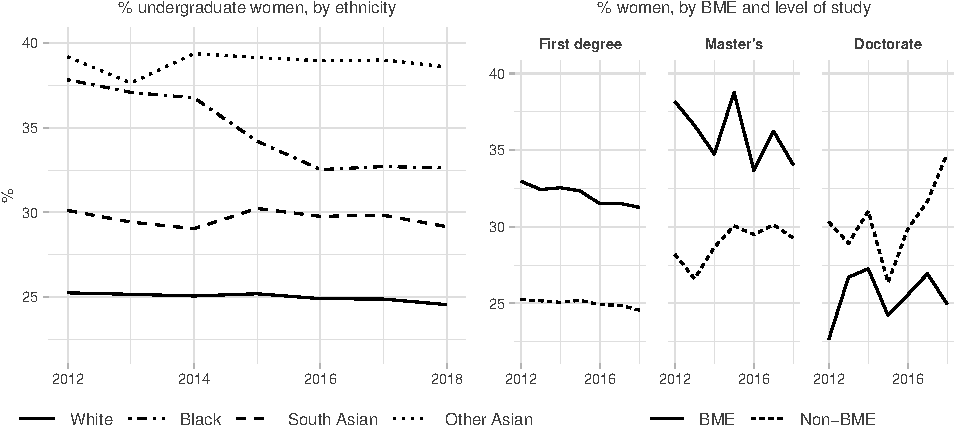
\includegraphics[width=\linewidth]{0-images/bme-1.pdf}

\caption{UK economics students, by ethnicity/BME marker}
\label{fig:bme}
\justify\footnotesize\textit{Note}.  Left-hand graph plots the percentage of female undergraduate economics students in the UK by ethnicity; right-hand graph plots the percentage of women among BME and non-BME students by level of study. Data are for full-time male and female students studying on a standard degree programme; left-hand graph excludes individuals whose ethnicity is unknown, other or mixed; right-hand graph excludes students with an unknown BME marker. See Appendix \ref{sec:data-definitions} for further information on how ethnicity was categorised. Data from HESA.
\end{figure}



Non-white women are more likely to study economics than white women. The left-hand graph in Figure \ref{fig:bme} plots the percentage of female undergraduate women by ethnicity.\footnote{The percentages of female students in Figure \ref{fig:bme} are lower (particularly at the master's level) than those shown in Table \ref{tab:contract} because non-UK domiciled students are disproportionately likely to have an unknown ethnicity, and are therefore not shown in Figure \ref{fig:bme}.} The representation of women is highest among ``other'' (\emph{i.e.}, non-South) Asian (39 percent) and Black (33 percent) students, although the percentage for Black students has declined 5 points since 2012. South Asian and white students have the lowest percentages of women: in 2018, only 29 and 25 percent, respectively. These patterns have remained relatively stable since 2012.

But while women are better represented among BME students than they are among non-BME students at the undergraduate and master's level, the reverse is true for Ph.D.~students. The right-hand graph in Figure \ref{fig:bme} plots the percentage of women by BME status and level of study. In 2018, the gaps between the shares of women among BME and non-BME students was 7 percentage points for students taking their first degree and 5 percentage points for master's students. Among doctoral students, however, the representation of women was 10 percentage points higher among non-BME students than it was among BME students.

The bottom two graphs in Figure \ref{fig:secondary} (Appendix \ref{sec:secondary}) plot the percentages of BME and non-BME economics undergraduate students who are women by type of secondary school and A-level subject. The percentage of women among BME students is higher than it is among non-BME students regardless of secondary school type or A-level subject. These patterns have not changed much with time; the exception is the percentage of BME students without an economics A-level that are women, which has declined from 37 percent in 2012 to 32 percent in 2018.

\hypertarget{sec:discussion}{%
\section{Discussion}\label{sec:discussion}}

According to our data, women comprise only 26 percent of academic economists in the UK. Unfortunately, representation is not radically higher elsewhere: women are also 26 percent of worldwide economists \citep{RePEc2022} and 26 percent of economists at Ph.D.~granting institutions in the United States \citep{Chevalier2021}. According to \citet{Auriol2022}, women are a slightly higher fraction (33 percent) of academic economists in continental Europe, although there is substantial heterogeneity across countries.

Our evidence also suggests that female economists in UK academia are promoted more slowly than male economists. Again, the trend is similar in most other countries \citep[see, \emph{e.g.},][]{Auriol2022, Ceci2014, Chevalier2021, Ginther2014, Jacobsen2006b, Lundberg2019}. In the United States, CSWEP tracks cohorts of Ph.D.~students through the academic pipeline; while women tend to achieve assistant professorships at the same rate as their male peers, this is not the case at higher academic ranks \citep{Chevalier2021, Lundberg2019}. Moreover, \citet{Ginther2004} found that only 47 percent of female economists were tenured 10 years post-Ph.D., compared with 68 percent of male economists.

We further find that growth in women's representation may be starting to slow, a long-term trend consistent with data from the United States \citep{Lundberg2019} and apparent in other metrics of gender inequality. Progress on women's representation in top economics journals has been particularly glacial, \emph{e.g.}, between 1986--2015, there was zero growth in the fraction of exclusively female-authored papers published in ``top-five'' economics journals \citep{Moon2022}.\footnote{The ``top-five'' journals in economics are the \emph{American Economic Review}, \emph{Econometrica}, \emph{Journal of Political Economy}, \emph{Quarterly Journal of Economics} and \emph{Review of Economic Studies}.} Even though the gender pay gap declined across Britain between 1999--2016, there was ``no notable fall in the unexplained (conditional) gender pay gap for UK academic economists'' during the same period \citep[p.~103]{Mumford2019}; at the London School of Economics, it actually increased \citep{Bandiera2016}.

In contrast, industry and government appear to have had more success at creating work environments that are attractive to female economists. In the UK Treasury, 38 percent of economic staff are women \citep{CabinetOffice2020}. At the Bank of England, 32 percent of senior staff and 46 percent of their new graduate intake are women \citep{BoE2020}. At the Institute for Fiscal Studies, 52 percent of in-house researchers are female \citep{IFS2021} and at NIESR, 45 percent are \citep{NIESR2021a, NIESR2021b}.

Why are women under-represented in academic economics and why has progress been so slow? As is well known, women face more obstacles on career progression---including gendered societal expectations regarding unpaid care---and the way academia responds to these obstacles (relative to other career options) may increase the opportunity cost of remaining. For example, \citet{Goldin2014} argues that many women prefer flexible work and are willing to sacrifice pay and promotion to achieve it. And although evidence does not suggest that flexibility is important to women early in their careers, it does suggest that they develop a revealed preference for it by the time they reach their 30s \citep{Ferriman2009, Lubinski2006, Ceci2014}. As a result, greater scope for part-time employment would likely encourage more women to remain in academia and may explain why industry and government have had more success attracting and retaining them.\footnote{A related barrier may be the fact that ``work devotion'' is a particular feature of academic life, with academics being ``especially responsive to the demands of work, because the success and rewards of their work are central to how they define themselves'' \citep[p.~3]{Fox2021}. \citet{Goldin2014} argues that the gender gap could be reduced considerably if employers ``did not have an incentive to disproportionately reward individuals who labored long hours'' \citep[p.~1091]{Goldin2014}. Increasing demands in terms of international travel---for conferences, collaborations and jobs---are a related feature of academic life \citep{Canibano2016}. This can offer opportunities to women, but it can also ``raise barriers''. \citet{Ferber1979} noted that three-quarters of women in the USA with Ph.D.s are partnered with someone who also has a Ph.D.~(whereas only a third of men with Ph.D.s are partnered with women with Ph.D.s), creating greater potential conflict in the careers of women. They further noted that women Ph.D.s are more likely to move for their partner's career (than vice versa), and that the more they do so, the lower are their own chances of being employed. Further research is needed on the degree to which this remains the case.}

Another issue stalling women in UK academia is discrimination related to pay and promotion. \citet{Bandiera2016} found that women earned 11 percent less than men at the London School of Economics, controlling for age, tenure and research productivity. \citet{Mumford2019} surveyed academic economists across the entire UK and found a gender pay gap of 9.1 log percentage points after conditioning on similar variables. \citet{McManus2018} analysed submissions for the UK's 2014 Research Excellence Framework and found that economics departments were about 10 percent less likely to submit research by female lecturers compared to observably equivalent male lecturers. In the United States, women take longer and are less likely to achieve tenure in economics, conditional on publication, citations and children \citep{Ginther2014}, and articles women co-author with men count less toward their promotion compared to articles men co-author with other men \citep{Sarsons2021}.

Evidence also suggests that female-authored articles are held to higher standards, potentially further limiting women's academic careers. Papers authored by women are 6.8 percent less likely to be accepted to conferences \citep{Hospido2021} and spend longer in peer review \citep{Hengel2022, Alexander2021}. Once published, they are more readable and receive more citations \citep{Card2020, Hengel2022, Moon2022, Grossbard2021}. Consistent with these findings, a controlled laboratory experiment found that ``female authors appeared to be seen as less competent than males, in that subjects (being incentivized to give their best judgement) less often believed that their papers have been published'' \citep[p.~326]{Krawczyk2016}.

Women economists also face more hostile working conditions compared to men. \citet{Wu2020} applied text mining and machine learning methods to posts on Economics Job Market Rumors (EJMR), a popular, anonymous online forum of economists. She found that posts about women were more focused on personal characteristics compared to posts about men, which tended to emphasise professional accomplishments. During seminars, female economists are also asked more questions, and a higher proportion of those questions are perceived as unfair, hostile or patronising by audience members \citep{Dupas2021}.\footnote{Growing concern about the treatment of women recently led the American Economic Association to survey their members about the professional climate in economics. The survey found that women were significantly more likely than men to say that they had personally experienced discrimination or unfair treatment with respect to pay, publishing decisions, invitations to conferences and networks, course evaluations and service obligations \citep{AEA2019}. Compared to men, women were also far less likely to agree with the statement ``I am satisfied with the overall climate within the field of economics''. In the UK, a similar climate survey was subsequently conducted by the Royal Economic Society. It found that 52 percent of respondents agreed that the climate in economics is aggressive and 32 percent that it is discriminatory \citep{RES2020}. Only one in three agreed or strongly agreed that it is inclusive.}

Economics' lack of diversity may arguably affect the way it is studied and its ability to attract a more diverse group of scholars going forward \citep{Bateman2019}. The majority of introductory economics courses still do not reference gender \citep{Asarta2020}, and the profession appears to have a particular ``resistance to any kind of feminist theory or feminist activism'' (Nancy Folbre, quoted in \citet{OrozcoEspinel2022}, p.~1186). Moreover, evidence suggests that topics of specialisation that disproportionately attract women or minorities are seen as lower status \citep{Key2019, Fortin2021, Zacchia2021}.\footnote{Relatedly, public goods disproportionately provided by women---including mentoring and diversity activities---are often undervalued in hiring and promotion decisions \citep[see, \emph{e.g.},][]{Jacobsen2006a}.} As a result, some may choose to eschew economics altogether (missing women) while others search for a scholarly home in non-economics departments (hidden women).

\hypertarget{sec:conclusion}{%
\section{Conclusion}\label{sec:conclusion}}

In this paper, we examine women's representation in UK economics, from the undergraduate level through to the professorship, over the period 1996--2018. We find that women now represent around a quarter of academic economists---33 percent of lecturers, 27 percent of senior lecturers/readers and 15 percent of professors---up from 18 percent in 1996.

But while progress has clearly been made, we also identify a number of ways in which women's representation may be stagnating and even retreating. To begin with, the academic pipeline is shrinking. Among UK nationals, the female proportion of economics students has fallen over the past two decades. In 2002, 31 percent of UK nationals studying economics at undergraduate level were women; by 2018, this had fallen to 27 percent. Once the intersection of gender and race is considered, we find even more cause for concern. While the proportion of women amongst minority groups is higher than it is among white students at the undergraduate level, the reverse is true for Ph.D.~students: women's representation in 2018 was 10 percentage points higher among non-BME Ph.D.~students than it was among BME Ph.D.~students. At the other end of the pipeline, there is a particular absence of non-white women. We could not find a single Black female professor of economics in the UK in the period up to 2018, and the proportion of women among professors with Asian ethnicity fell from 22 percent in 2012 to 16 percent in 2018.

Our findings for the UK are not unlike those elsewhere in the world and add to a growing literature documenting academic gender gaps. In addition to a lack of representation, women are paid less and are less likely to achieve tenure or be promoted compared to their male peers. They are also given a harder time in seminar presentations and are substantially less likely to publish in top economics journals.

One question we have not explored is whether women are ``missing'' from the economics profession entirely or just ``hidden'' from view. Given the historic purpose of the RES's data collection efforts, we have narrowly defined ``economists'' to include only academics studying or working in economics departments or business schools. As a result, we have, sadly, overlooked female economists in departments excluded by this definition---\emph{e.g.}, history, political science or sociology. We hope future research will more carefully investigate whether female economists are ``missing'' from the academy entirely, or instead simply ``hiding'' in economics-adjacent disciplines.

\newpage

\hypertarget{references}{%
\section*{References}\label{references}}
\addcontentsline{toc}{section}{References}

\bibliography{0-bib/references}

\newpage

\hypertarget{appendix-appendix}{%
\appendix}


\setcounter{figure}{0}
\setcounter{table}{0}
\setcounter{equation}{0}
\counterwithin*{table}{section}
\counterwithin*{figure}{section}
\renewcommand{\thetable}{\thesection.\arabic{table}}
\renewcommand{\thefigure}{\thesection.\arabic{figure}}
\appendixpage

\hypertarget{sec:data-definitions}{%
\section{Data definitions}\label{sec:data-definitions}}

\hypertarget{staff-definitions}{%
\subsection*{Academic staff}\label{staff-definitions}}

For staff members, we concentrate our analysis on sex, academic rank, academic employment function, part-/full-time employment status, terms of employment, nationality and ethnicity. Below we briefly describe data definitions; more detailed information is available on \href{https://www.hesa.ac.uk/support/definitions/staff}{HESA's website}.

\begin{itemize}
\item
  Sex refers to the sex of the individual as opposed to the gender they identify with. HESA data include three gender categories: male, female and other. In the present analysis, we specifically exclude individuals who do not declare their gender as either male or female. (Given other data restrictions, however, all staff observations are either male or female, anyway.)
\item
  Academic rank (or contract level) records the UCEA or XpertHR defined level of the contract. In most analyses, we only include levels F1 (professor), I0 (senior lecturer/reader), J0 (lecturer B) and K0 (lecturer A).\footnote{See Footnote \ref{fn:lecAB} for the distinction between ``lecturer A'' and ``lecturer B'' positions.} In Section \ref{sec:staff-temp}, we also include L0 (teaching and research assistants).
\item
  Academic employment function refers to the role/categorisation of an academic contract (teaching only, teaching and research or research only); staff members without teaching or research responsibilities are excluded from all analyses.
\item
  Part-/full-time status is attributed to the contract; thus, an individual working full time on multiple part-time contracts would be represented as multiple part-time instances in the data.
\item
  Terms of employment describe the type of contract an employee holds (open-ended/permanent or fixed-term); all analyses exclude staff members employed on atypical contracts.
\item
  Nationality refers to the country of legal nationality.
\item
  Ethnicity data are voluntarily self-reported according to the coding framework recommended by the Office for National Statistics. To comply with HESA's rounding and suppression strategy, we categorise the ethnicity of academic staff as follows: ``white'' includes individuals from any white ethnic background; ``Black'' includes individuals from a Black Caribbean, Black African or other Black background; and ``Asian'' includes individuals from an Indian, Pakistani, Bangladeshi, Chinese or other Asian background.
\end{itemize}

\hypertarget{students-definitions}{%
\subsection*{Students}\label{students-definitions}}

For students, we concentrate much of our analysis on sex, level of study, nationality, domicile, state school marker, A-level subject, ethnicity and BME marker. Data descriptions not already defined above for academic staff are briefly summarised below; for further details, please consult \href{https://www.hesa.ac.uk/support/definitions/students}{HESA's website}.

\begin{itemize}
\item
  Level of study refers to either undergraduate (first-degree) or postgraduate (master's or doctorate) study. Students studying on non-first-degree undergraduate programmes or non-master's/doctorate postgraduate programmes are omitted from all analyses.
\item
  Domicile refers to the location of a student's permanent home address prior to starting study.
\item
  State school marker indicates whether a student obtained his or her secondary education from a state school or a privately funded school or college.
\item
  A-level subject indicates whether the student obtained pre-university qualifications (also known as ``A-levels'' in the UK) in economics or not.
\item
  Student ethnicity is categorised as follows: ``white'' includes individuals from any white ethnic background; ``Black'' includes individuals from a Black Caribbean, Black African or other Black background; ``South Asian'' includes individuals from an Indian, Pakistani or Bangladeshi background; and ``Other Asian'' includes individuals from a Chinese or other Asian background.
\item
  Black and minority ethnicity (BME) marker indicates whether a student's ethnicity is categorised as either Black, Asian, Mixed or Other.
\end{itemize}

\newpage

\hypertarget{sec:temp-appendix}{%
\section{Staff on fixed term contracts}\label{sec:temp-appendix}}



\begin{figure}[h!]
\centering
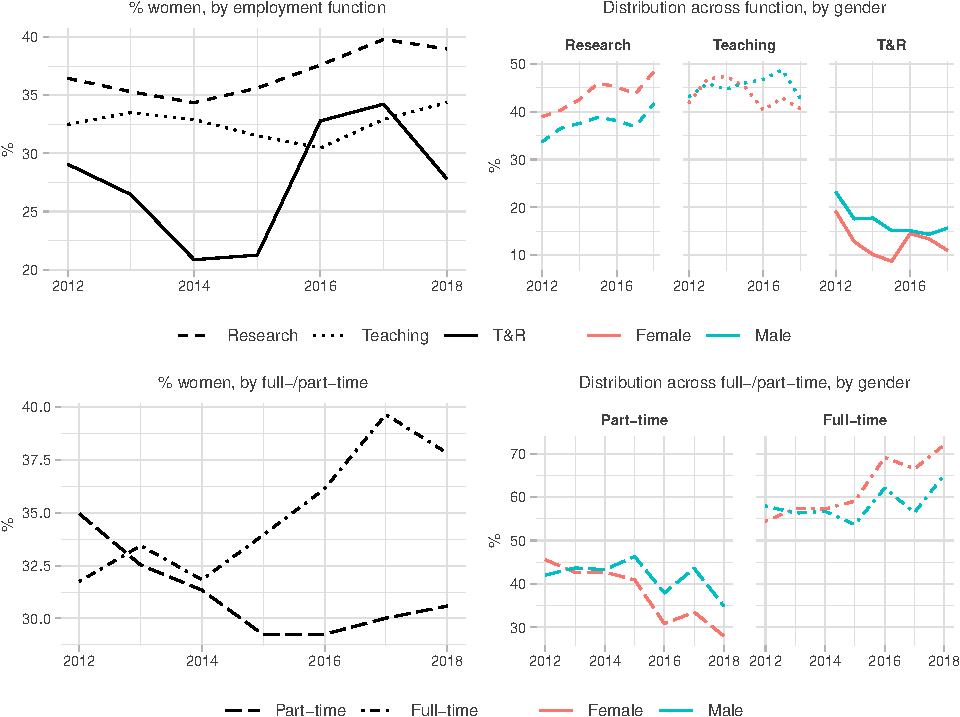
\includegraphics[width=\linewidth]{0-images/fixed-term-2-1.pdf}

\caption{UK academic economists on fixed-term contracts, by function and part-time status}
\label{fig:fixed-term-2}
\justify\footnotesize\textit{Note}.  Top left-hand graph plots the percentage of academics on fixed-term contracts who are women, broken down by academic employment function; top right-hand graph shows the percentages of all women and all men on fixed-term contracts across academic employment function. Bottom left-hand graph plots the percentage of academics on fixed-term contracts who are women, broken down by full- and part-time status; bottom right-hand graph shows the percentages of all women and all men on fixed-term contracts across full-/part-time status. Data restricted to academic economists (including teaching/research assistants) working both full- and part-time in teaching-only, research-only or T\&R positions. Data from HESA.
\end{figure}



\newpage

\hypertarget{sec:student-nationality}{%
\section{Students' nationality}\label{sec:student-nationality}}



\begin{figure}[h!]
\centering
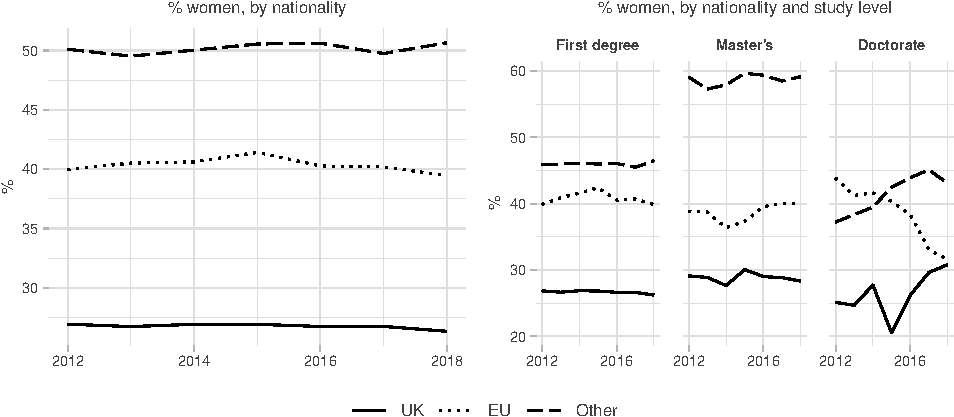
\includegraphics[width=\linewidth]{0-images/domicile-2-1.pdf}

\caption{UK economics students, by nationality}
\label{fig:domicile-2}
\justify\footnotesize\textit{Note}.  Left-hand graph plots the percentage of female students in economics by nationality; right-hand graph plots the percentages of women, by study level and nationality. Data are for full-time male and female students studying on a standard degree programme; students with unknown nationality are excluded. Data from HESA.
\end{figure}



\newpage

\hypertarget{sec:secondary}{%
\section{Students' secondary education provider}\label{sec:secondary}}



\begin{figure}[h!]
\centering
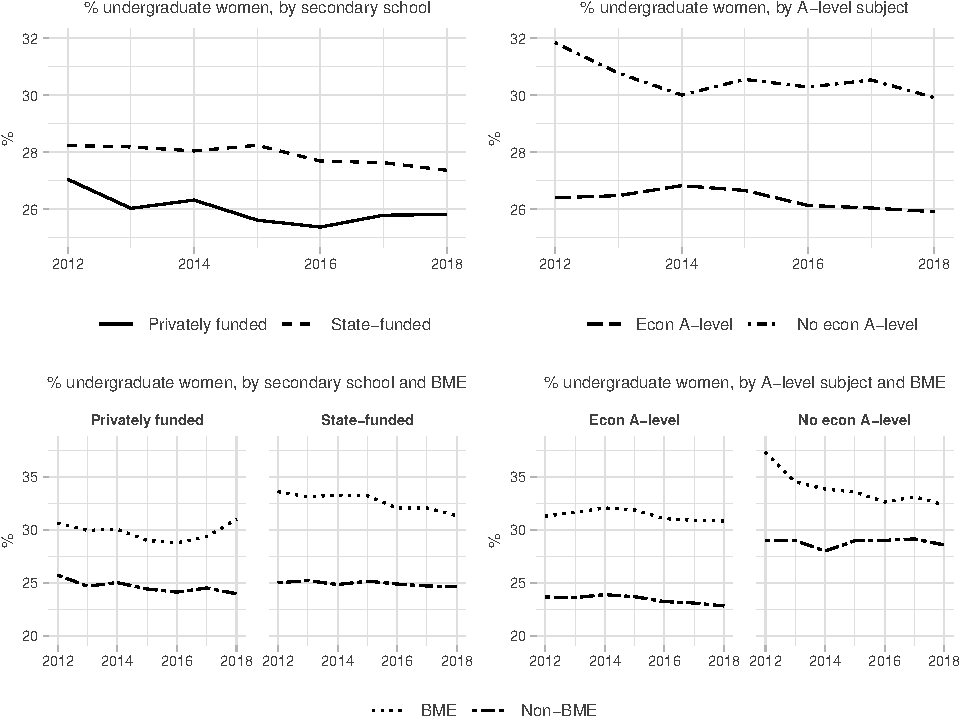
\includegraphics[width=\linewidth]{0-images/secondary-1.pdf}

\caption{UK economics students, by secondary education and BME marker}
\label{fig:secondary}
\justify\footnotesize\textit{Note}.  Top left-hand graph plots the percentage of female undergraduate economics students by type of secondary school; top right-hand graph plots the percentage of female economics undergraduates by A-level subject. Bottom left-hand graph shows the percentages of undergraduate women studying economics by BME marker and type of secondary school; bottom right-hand graph shows the percentages of undergraduate women by BME marker and A-level subject. Data are for full-time male and female undergraduate students domiciled in the UK studying on a standard degree programme. Data omit students with an unknown type of secondary school (left-hand graphs only), A-level subject (right-hand graphs only) and BME marker (bottom two graphs only). Data from HESA.
\end{figure}




\end{document}
